Karma takes the user's selected properties, e.g. the artist's biography (for completeness) and birth (for validation), and searches for matching triples.
Karma then merges the results and updates the source model appropriately as illustrated in Figure~\ref{fig:augment-screenshot}, so the user can continue to explore the integrated data interactively. 

\begin{figure*}
\begin{center}
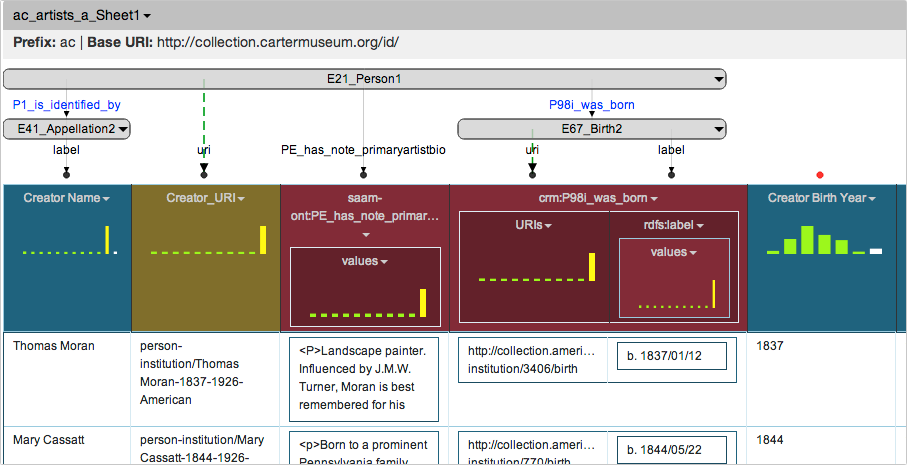
\includegraphics[width=4.9in]{images/6-augment.png}
\vspace{-3mm}
\caption{A Karma user has integrated biographical data from the Smithsonian into their dataset}
\vspace{-2mm}
\label{fig:augment-screenshot}
\end{center}
\vspace{-1.5em}
\end{figure*}
